\documentclass[a4paper]{article}

\usepackage[utf8]{inputenc}
\usepackage[T1]{fontenc}
\usepackage[english]{babel}

\usepackage[hidelinks]{hyperref}
\usepackage{graphicx}

\title{{\Huge Image Search} \\[1cm] Project in DD2476 Search Engines and Information Retrieval Systems \\[1cm] }
\author{ 
    Tobias Andersson <\href{mailto:tobias2@kth.se}{tobias2@kth.se}> \and
	Florian Carra <\href{mailto:fpcarra@kth.se}{fpcarra@kth.se}> \and
	Daniel Forslund <\href{mailto:dforsl@kth.se}{dforsl@kth.se}> \and
    Jonas Sköld <\href{mailto:jonassko@kth.se}{jonassko@kth.se}> \and
    Martha Vlachou-Konchylaki <\href{mailto:marthavk@kth.se}{marthavk@kth.se}>
}
\date{\today}

\begin{document}

\maketitle
\thispagestyle{empty}

\clearpage

\begin{abstract}
This is a study about the possibilities of creating a useful image search engine that indexes images based on their surrounding context. We have created a search engine which searches images on English Wikipedia and assessed its performance on different kinds of search queries. The performance was decent overall, but varied greatly between different search queries. The filename and alt-tag of images, as well as the title of the page it appears on, was found to be most important for generating good search results. However, this was not true for all types of queries. 
\end{abstract}

\vspace{1cm}

\tableofcontents

\clearpage

\section{Introduction}

Searching for content on the web is becoming an increasingly important part of daily life. We are in the middle of a search revolution, which is evident when looking at Google's usage statistics. Last year, Google alone accounted for 25\% of all internet traffic in North America. In 2010 the same number was only 6\% \cite{google-traffic}. On top of that, Google receives over 3 billion queries per day world wide \cite{google-searches}. Most of those queries are no doubt queries for text, but a text result is not always sufficient. Image results brings a different perspective on information retrieval, and that is the focus of this project. As opposed to a regular search engine that returns text documents that are deemed relevant to the text query, image retrieval systems return images.

\subsection{Problem Statement}
Our task is to build an image search system and to evaluate it. The evaluation will aim to answer the question: How does the weighting of the search fields affect different queries?

In order to limit the indexing scope of our search engine, only articles on English Wikipedia will be indexed.

\subsection{Background} 
The history of information retrieval systems did not begin with web search systems. The earliest computer-based search systems were introduced in the late 1940s. Back then only text was interesting to search for, as computers could not display graphics. The history of image retrieval begins in the 1970s and has, since then, been an active research area. \cite{ir-history}

The issue that separates image retrieval from text search is that each word in a text is easily distinguishable and can be indexed directly. Finding an image based on a query composed of text is a more difficult task. There are two schools of image retrieval systems which tackle this problem in their own way: one based on indexing text related to the image and one based on analyzing the image content, i.e. trying to identify visual features that can be connected to a query term. Such visual features are colors, shapes and textures. This project will focus on the former school while our approach relies on indexing the surrounding text and meta-data of the image. \cite{image-retrieval-history} 

When using textual information, many useful techniques used in general information retrieval systems can be applied, such as stemming. A stemmer is reducing words to their base form before indexing and/or before a query is processed, resulting in increased recall at cost of reduced precision. Another technique is to use a synonym dictionary to add synonyms of the query terms to the query, or to exchange all words to one of its synonyms. \cite{stemming} \cite{expansion}

\subsection{Related work}
Most successful image search engines take advantage of both textual and content-based information. WebSeer, one of the earliest image retrieval systems for the World Wide Web combined surrounding text and image content cues for an optimal implementation \cite{WebSeer}. The Chabot project initiated at University of California, also points out the significance of combining the two approaches \cite{Chabot-project}.

Technical tools such as database organization are also central to studies based on image search engines. A patent led by Jeffrey R Bach and Bradley Horowitz\cite{database-indexing} states that only few discriminant criteria are used for each different query. By indexing specificities for each criteria, we are able to use only relevant fields for a given query, which leads to a significant improvement of space and time complexities.
 
\section{Method}
This section is divided into two parts: the first elaborates on the different parts of our search engine while the second describes our experiments.

\subsection{Implementation}
There are two main processes in the search engine: the indexing and the search process. The indexer is not dealing with image processing like object recognition, color analysis etc. thus the data about an image is limited to its related text, i.e.  the file name, description, and adjacent text. 

The indexing process is divided into several modules that communicate with each other. The first step is a web crawler that starts at a page and follows all links on the pages it visits. Our crawler was configured to start at the main page of Wikipedia. The second step is an HTML parser which fetches relevant information from each of the pages that the crawler visits. The parser then sends the data to an Apache Solr database through a connector. Solr handles the indexing of the parsed image information.

The search process is a web application that queries the Apache Solr database and displays the most relevant images. The application also lets the user decide on which parts of the Wikipedia content that should be most important in the search, for instance the image caption or the surrounding text.


\subsubsection{Crawler}
The first step towards indexing images in Wikipedia articles is to find the correct documents and pass them to a parser. For this purpose a web crawler was used. A web crawler is a program that starts at a specific web page, called a seed, and follows all URLs from the seed. It then proceeds to recursively visit the pages linked by each page it visits, if the link matches the crawler's visitation policy. In our case the seed is the home page of English Wikipedia, and the visitation policy is that only web pages that are English Wikipedia articles are visited, that is URLs that start with: \url{http://en.wikipedia.org/wiki/}. Additionally the crawler was configured to visit a maximum of 100 000 articles. Each page that is visited is downloaded and sent to the parser for processing. The web crawler Crawler4j\footnote{Available from: \url{https://code.google.com/p/crawler4j/}} was was chosen because it is easy to use, open source, and written in Java, like the rest of the tools used in this project. 

\subsubsection{Parser}
The parser is designed to work on Wikipedia pages. All Wikipedia pages have roughly the same structure, which makes it easy to parse the pages and find relevant data. There are mainly two different locations at which images are positioned on a Wikipedia page. The first location is in the top right corner, in an "info box". There can be multiple images in the info box, and some pages have no images at all in this location. The second position is "inline" in the running text. These images are often associated with the adjacent text, so that text potentially describes the image quite well.

A parsing library called jsoup is used which is an open source java library for HTML parsing \cite{jsoup}. It uses css-selector syntax to find interesting elements in the web page. When knowing the structure of a page in advance, as is the case when parsing only Wikipedia pages, css-selector syntax is an easy way of parsing a HTML file.

The parser finds seven different texts, or attributes, for each image on a page. Three of them are taken straight from the image tag. These are url, file name and alt attribute. The file name is just the url without the leading path and the file extension, and underscores and hypheens have been replaced with spaces to separate the words in the file name. A fourth attribute of the image is description, which is the short text immediately following the image, also known as image caption. The fifth field is the context of the image. This is the paragraph adjacent to the image. For the images in the top right info box, the first paragraph of the page is used as the context. For images in the running text, the first paragraph after the image is used. The last two fields are the title and subtitle. The title is simply the title of the Wikipedia article, and the subtitle is the title of the section in which the image is located. Not all of these fields can be found for each image. For instance, images on Wikipedia often lack the alt attribute, some do not have a caption, and the images in the info box do not have a subtitle.


\subsubsection{Apache Solr}
When Apache Solr receives documents containing image information, it will immediately index it and add it to its database. The index is made of documents, where a document corresponds to a specific image. There are 6 fields in the index used when searched that come immediately from the parser. These are an image's file name, alt attribute, description, context, its page's title and subtitle. In addition to these, there is a catch-all field which contains the data of all fields and a catch-all field in reverse. 

Also, stemming is applied on the index side. There are different kinds of stemming strategies, but the one used is stemming by reduction. This means that words will be reduced to their stem or root. For instance, a stemmer for English should identify words such as "walks, walking, walked" as based on the root "walk" and "fishing" as "fish". 

When a search is being carried through, there are three important aspects of the used configuration. A search query is received containing general tokens to search for and possibly some that are field-specific. The documents (images) are scored using tf-idf, which is a numerical statistic which reflects the importance of a word in a document. "tf" correlates to a term's frequency, the number of times it occurs in the currently scored document. A document containing more occurrences of a given term receives a higher score. The "idf" part stands for inverse document frequency and is a measure of how rare the term is across all documents. Rarer terms give higher contribution to the total score. The number of query terms found in a document is also taken into consideration, so that documents containing more of the query's terms receive a higher score than documents containing fewer query terms.

In addition to the query, the configuration instructs Apache Solr to take optional weights of the different fields into consideration when calculating scores. For instance, assigning the weight 2.4 to field1, 0.4 to field2 and 1.1 to field 3 tells Apache Solr that field1 is of much higher importance than field2 and field 3. Of the three fields, field2 is the least important one and it will contribute less to the score of a document.

As the indexing process includes stemming by reduction, this must also be done for the queries to be able to find a match.

\subsubsection{Web Application}
The web application allows the user to search any image stored in the Apache Solr database through text queries. Queries can be made of simple tokens, for instance "Barack Obama" or "blue shirts", typed into a simple text field. They can however also target specific data fields of the image, such as the Wikipedia page title or the image's alt attribute. Apart from specifying queries, the application also allows the user to add weights to the different data fields. Adding a weight to a data field instructs Apache Solr to increase the score for images with matchings in the specific field. 

When the search result is returned from Apache Solr, it is displayed and ordered by descending score. All information regarding the image is also available to the user when inspecting the image, which is done by clicking it. The communication with Apache Solr is carried through its REST-like JSON API over HTTP.

\subsection{Experiments}
Our next task was to develop a framework for experimentation on the final behaviour of the search engine. The idea is to set weights on every field and alternate them in order to observe how each element affects the quality of the search by calculating the precision at 10 for each configurations. Our web interface served as a visualization tool allowing easy adjustment of the weights. As the total number of relevant documents (images) in the index was not known the recall of the search results could not be calculated.

We decided to observe the results of 10 queries with different properties. Our test queries were:

\begin{enumerate}\and
  \item Barack Obama
  \item Summer
  \item Blue Sky
  \item Cat
  \item War On Terror
  \item Great Britain
  \item International Space Station
  \item Camping
  \item Airplane
  \item Brown Hair
\end{enumerate}	

As far as the weight settings are concerned, the values of each weight varies between 1 and 10. 
Each query was searched using the following weight configurations: 
\begin{description}
  \item[No Configuration:] The weights were all set to 1. 
  \item[Metadata:] Importance was given to the fields related to the metadata of the image. More specifically the   \textbf{Filename} and \textbf{Alt-tag} values were set to 10 while all other remained at 1.
  \item[Context:] Here the fields containing information about the context of the image were given a greater importance. The weights for this configuration were set as follows: \textbf{Description} and \textbf{Title} fields were weighted by 10 while \textbf{Content} and \textbf{Subtitle} were given a value of 5.
  \item[Optimal Configuration:] For each query we tried to find the weight adjustment that yields the best performance. This configuration is different for the type of each query and is presented in the next section. 
\end{description}

\begin{figure}
\begin{center}
\begin{tabular}{| l || c | c | c | c | c | c |}
\hline
                                 & filename & alt-tag & description & context & title & subtitle \\ \hline
 No Configuration     & 1 & 1 & 1 & 1 & 1 & 1 \\ \hline
 Metadata                 & 10 & 10 & 1 & 1 & 1 & 1\\ \hline
 Context                    & 1 & 1 & 10 & 5 & 10 & 5 \\ \hline
\hline
\end{tabular}
\caption {Weight settings for different configurations}
\label{weightconfig}
\end{center}
\end{figure}

%%No Configuration & Metadata & Context \\ \hline

\section{Results}
This section presents the results of the experiment described above. Figures \ref{precision} and \ref{optvect} depict the precision (number of relevant documents) of the engine for the first 10 images of the retrieved list and the weight vectors which resulted in the best performance respectively. 
The number of parsed pages was 100.000 from which 400.000 images were indexed. 

\begin{figure}
\begin{center}
\begin{tabular}{ c | c }
\\
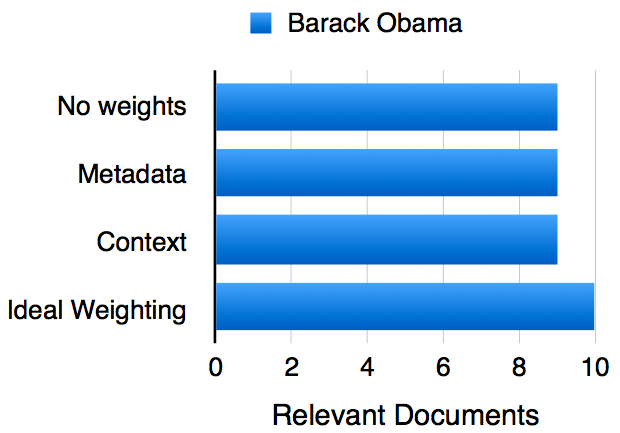
\includegraphics[width=0.4\textwidth,height=10em]{01BarackObama} & 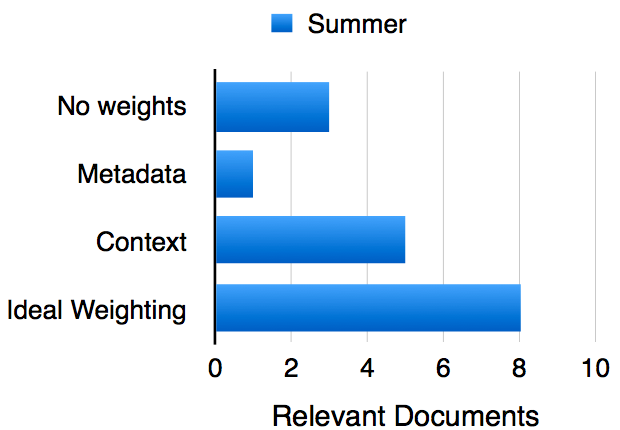
\includegraphics[width=0.4\textwidth,height=10em]{02Summer} \\  \hline \\
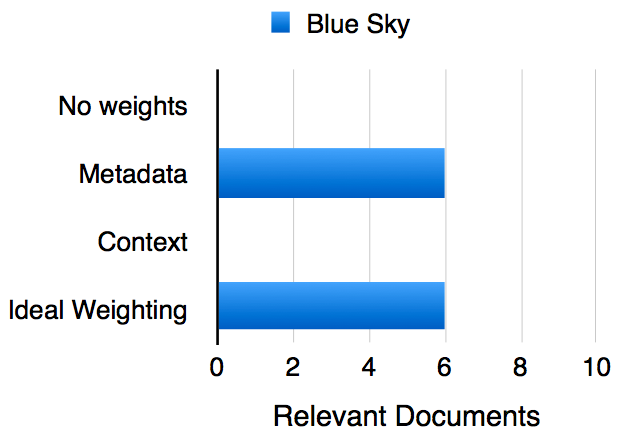
\includegraphics[width=0.4\textwidth,height=10em]{03BlueSky} &
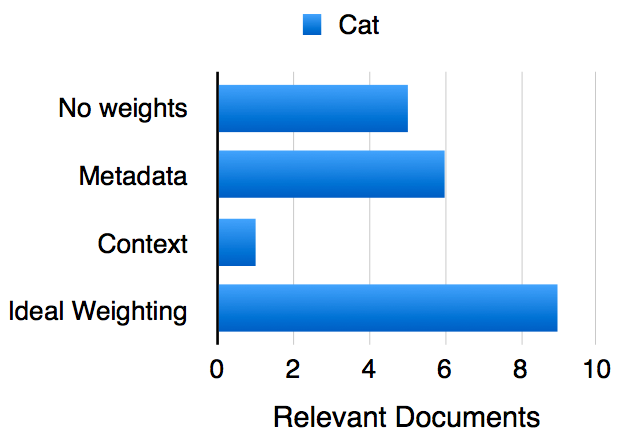
\includegraphics[width=0.4\textwidth,height=10em]{04Cat} \\  \hline \\
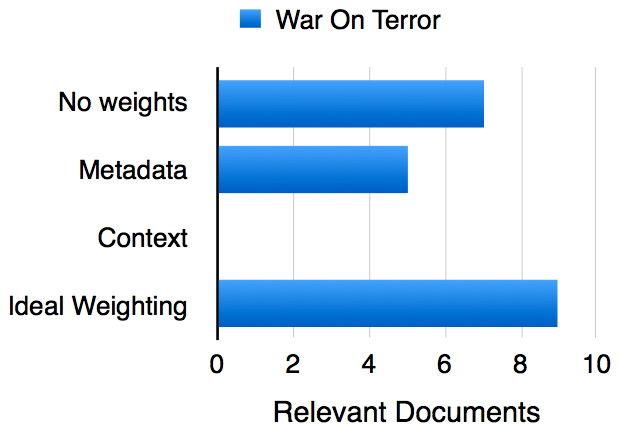
\includegraphics[width=0.4\textwidth,height=10em]{05WarOnTerror} &
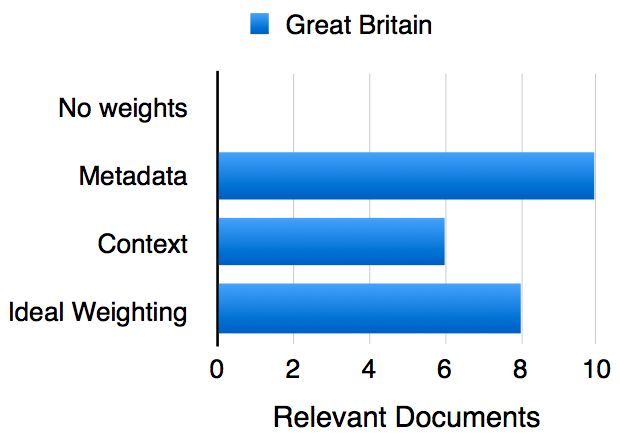
\includegraphics[width=0.4\textwidth,height=10em]{06GreatBritain}  \\ \hline \\
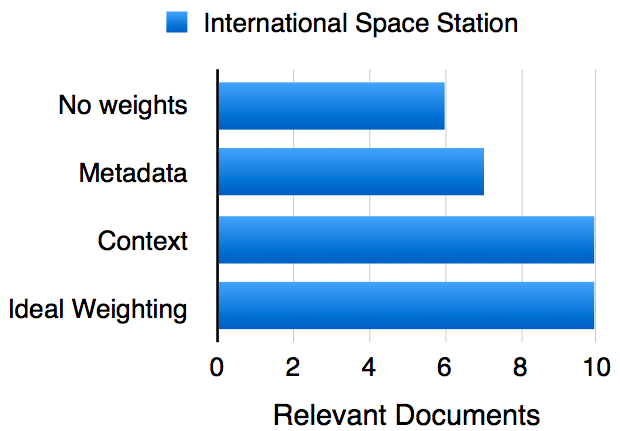
\includegraphics[width=0.4\textwidth,height=10em]{07InternationalSpaceStation} &
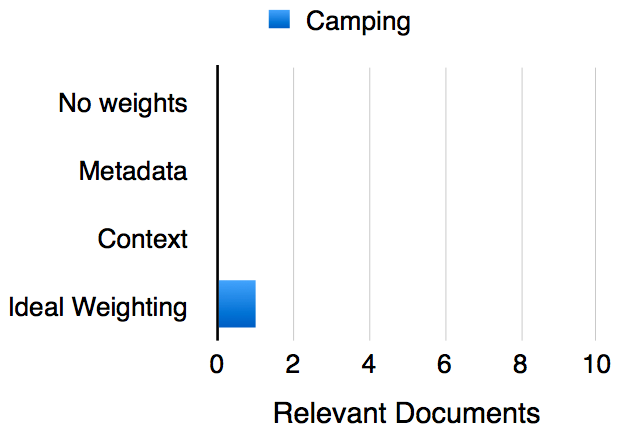
\includegraphics[width=0.4\textwidth,height=10em]{08Camping} \\ \hline \\
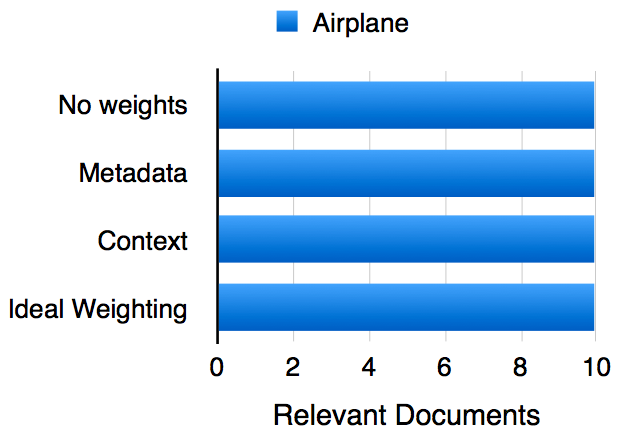
\includegraphics[width=0.4\textwidth,height=10em]{09Airplane} &
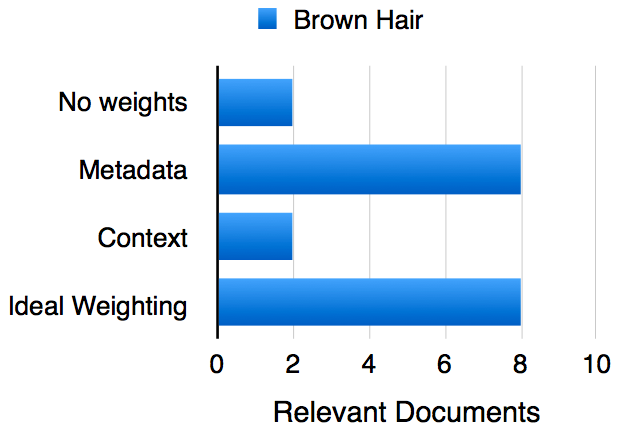
\includegraphics[width=0.4\textwidth,height=10em]{10BrownHair} \\ 
\end{tabular}
\caption{Precision for the ten queries}
\label{precision}
\end{center}
\end{figure}

\begin{figure}
\begin{center}
\begin{tabular}{| l || c | c | c | c | c | c |}
\hline
                                 		& filename & alt-tag & description & context & title & subtitle \\ \hline
 Barack Obama   		& 10 & 1 & 1 & 1 & 1 & 1 \\ \hline
 Summer   				& 10 & 1 & 5 & 5 & 10 & 1\\ \hline 
 Blue Sky 				& 10 & 10 & 1 & 1 & 1 & 1\\ \hline 
 Cat 					& 10 & 5 & 10 & 6 & 5 & 6\\ \hline 
 War On Terror 			& 5 & 5 & 5 & 5 & 1 & 5\\ \hline
 Great Britain 			& 10 & 1 & 1 & 1 & 1 & 1\\ \hline
 International Space Station& 1 & 1 & 1& 1& 10 & 10\\ \hline
 Camping 				& 5 & 1 & 5 & 1 & 1 & 1\\ \hline
 Airplane 				& 1 & 1 & 1 & 1 & 10 & 10\\ \hline
 Brown Hair 			& 1 & 10 & 1 & 1 & 5 & 5\\ \hline
\hline
\end{tabular}
\caption{Ideal weight configurations for the ten queries}
\label{optvect}
\end{center}
\end{figure}

\section{Discussion}

In this project we specify a method for conducting web image search using image meta-data and surrounding text permitting variations on the weight of each element on the search. Our approach is aiming on detecting the useful information surrounding an image in order to increase the quality of the search.

Our results indicate that in most of the cases our simple weight configurations perform better than an unweighted configuration. However, the optimal weight configuration are not the same for each type of query. While the file name is the most important field in most cases, it was set to 1 in the optimal configurations of some queries, such as brown hair. This is because most relevant pictures other, more relevant information about the picture in the file name, such as the persons name. In this case the alt-tag did however prove to be very helpful as it contains a description such as "A photo of a woman with brown hair." on all the top results, while the file name contained the name of the person.

One reason why our relatively simple search engine still achieved very high precision for most queries is the simplified scope of out project: we only index Wikipedia articles. If we had to index the whole web, our search engine would encounter two main issues: file names and page structure. File names on Wikipedia often describe the image quite well. This is generally not the case on the web where and file names such as “DSC00125” or “image002” are very common. Another advantage of Wikipedia articles are their structure, which also facilitates extraction of image descriptions and context.

\subsection{Difficulties and Problems}	
While conducting our experiments we encountered two types of problems which caused a decreased performance:

Our relevancy ranking of search results was binary, i.e. an image is either relevant or not relevant. This made it easy to compare results and to produce charts. However in practice, image relevancy is not binary. For instance, searching for airplane may return both an image of a real airplane as well as a small airplane icon. Even though both images are relevant, the first image is arguably a better search result than the second. This was evident when trying to find the best weights for a query. One weight distribution could result in ten barely relevant images, giving a precision of 10 out of 10. Another distribution could also result in a 10 out of 10 precision, but all the images were highly relevant. Even though the second result was more satisfying, there is no difference between those results in the statistics.

What is more, the stemming process carried on both the index and queries is, as explained, stemming by reduction. It is a good strategy to unify words of the same stem, but it does also take the term out of context. For instance, searching for "fishing" will be translated into "fish" and could thus return a result set of images containing fish instead of, perhaps, people fishing. To compensate for this and further improve the search engine, a related technology that could have been used is lemmatization. This allows for "stemming" by expansion, taking a root word and "expanding" it to all of its various forms. Also, this could be done either at insertion time or at query time. As an example, lemmatization would group "walk" and "walking" as well as "good" and "better". 

\subsection{Future Improvements}
By examining the encountered problems and the final outcome of our search engine we can observe that there is a variety of directions for improvement. Our approach relies on images parsed from the Wikipedia web pages while a more large-scaled search, containing other types of websites with less structured content is seen prospectively as a challenge. The performance of the engine can be also increased elaborating towards content-based information retrieval \cite{cbmir}  or a combination of text and image analysis \cite{WebSeer}.


Other approaches include Natural Language Processing allowing for query or index expansion through classes or synonyms resulting in significant quality improvement in image search \cite{NLP}.

%There is a way to process text we index in order to get more than only a series of words. This solution is called NLP, for Natural Language Processing. A first step is known as POS (Part-Of-Speech). A POS Tagger will process a text to sort each of its constitutive word in a grammatical category (noun, adjective, adverb…). From this analysis, you can index more information related to specific words such as nouns or adjectives. By linking it to synonym dictionary, you are able to index more words related to the image, and therefore improve your accuracy. By defining relations between classes of words, you may significantly link group of words together. Relations are for example \cite{NLP} “AND-distribution”, “WITH-transitivity”, “WITH-distribution”… 

\section{Conclusion}
For precise queries, the biggest amount of information relies on the file name field. However, as queries become more abstract, content fields such as Title and Subtitle gain importance. Images corresponding to vague queries can be retrieved through the alt-tag field which contains an objective description of the image. However, the information included in these fields depend strictly on the format of the Wikipedia website. Indexing and retrieving images from the wider web as well as reconfiguring the weights to match a more general type of data is seen as a future challenge and may require content based analysis or natural language processing of the surrounding text.

\section{References}

\begin{thebibliography}{99}

\bibitem{google-traffic}
R. Mcmillan. Google Serves 25 Percent of North American Internet Traffic. 2013 Jul 22 [cited 2014 May 14]. Available from: \url{http://www.wired.com/2013/07/google-internet-traffic/}

\bibitem{google-searches}
English Wikipedia. Google Search. 2014 May 14 (latest revision) [cited 2014 May 14]. Available from: \url{http://en.wikipedia.org/wiki/Google_Search}

\bibitem{ir-history}
M. Sanderson, W. B. Croft. The History of Information Retrieval [Internet].  [cited 2014 May 14]. Available from: \url{http://ciir-publications.cs.umass.edu/getpdf.php?id=1066}

\bibitem{image-retrieval-history}
Y. Rui, T. S. Huang. Image Retrieval: Current Techniques, Promising Directions, and Open Issues. 1999 Jan 29 [cited 2014 May 14]. Available from: \url{http://www.cs.princeton.edu/courses/archive/spr05/cos598E/bib/rui99_cbir_survey.pdf}

\bibitem{WebSeer}  
Charles Frankel, Michael J. Swain, and Vassilis Athitsos. "WebSeer: An Image Search Engine for the World Wide Web." Chicago. August 1, 1996. Available from: \url{http://citeseerx.ist.psu.edu/viewdoc/download?doi=10.1.1.79.8996&rep=rep1&type=pdf} 

\bibitem{stemming}
English Wikipedia. Stemming. 2014 May 10 (latest revision) [cited 2014 May 14]. Available from: \url{http://en.wikipedia.org/wiki/Stemming}

\bibitem{expansion} English Wikipedia. Query Expansion. 19 Mar 2014 (latest revision) [cited 2014 May 14]. Available from: \url{http://en.wikipedia.org/wiki/Query_expansion}

\bibitem{Chabot-project}
Virginia E. Ogle, Michael Stonebraker. "Chabot: Retrieval from a Relational Database of Images". Berkeley. Available from: \url{http://citeseerx.ist.psu.edu/viewdoc/download?doi=10.1.1.64.989&rep=rep1&type=pdf}
\bibitem{database-indexing}
Jeffrey R Bach, Bradley Horowitz. "Indexing method for image search engine." Octroi. US6084595 A. Available from: {http://www.google.com/patents/US6084595}
\bibitem{jsoup}
Jsoup Java HTML Parser \url{http://jsoup.org}
\bibitem{cbmir}
Michael S. Lew. "Content-based multimedia information retrieval: State of the art and challenges". ACM Trans. Multimedia Comput. Commun. Appl. 2006. Available from \url{http://cmapspublic3.ihmc.us/rid=1228287418184_589199499_15410/content%20based%20multimedia.pdf}
\bibitem{image-processing}
Rohini K. Srihari, Debra T. Burhans. "Visual Semantics: Extracting Visual Information from Text Accompanying Pictures". 1994. Available from \url{https://www.aaai.org/Papers/AAAI/1994/AAAI94-121.pdf}
\bibitem{NLP}
Katerina Pastra, Horacio Saggion, Yorick Wilks. “NLP for Indexing and Retrieval of Captioned Photographs” University of Sheffield. Available from \url{http://aclweb.org/anthology//E/E03/E03-1065.pdf}



%%%%%%%%%%%%%%%%%
%%%% EXAMPLE %%% use \cite{users-manual} to refer to this source:
%
% \bibitem{users-manual}
% Chen M, Foroughi E, Heintz F et al. RoboCup Soccer Server [Internet]. 2002 Aug 2 [cited 2013 Mar 15]. Available from: \url{http://wwfc.cs.virginia.edu/documentation/manual.pdf}
\end{thebibliography}

\end{document}
